\chapter{قياس الزمن}\label{ch:g2:measuring-time}

``خمس دقائق أخرى فقط!'' --- لكن كم تبلغ هذه حقًّا؟ الزمن لا يُرى
ولا يُمسك ولا يُمدّ على مسطرة. ومع ذلك نقيسه كل يوم: فللسباقات
فائزون، والكعك يخرج لا نيئًا ولا محترقًا، والمدرسة تنتهي في اللحظة
الصحيحة. فلنتعلّم كيف يُروَّض الزمن.

\section{اللحظات والمُدد}

\begin{example}[ترتيب اليوم]\label{ex:g2:measuring-time:order}
اليوم موكب من الأحداث، على ترتيب واحد دائمًا: الاستيقاظ، فالفطور،
فالمدرسة، فالغداء، فبعد الظهر، فالعشاء، فالنوم. و``الفطور
\emph{قبل} المدرسة'' و``العشاء \emph{بعد} الغداء'' --- فالقبل
والبعد أول كلمتين في الزمن، مثلما كان الأطول والأقصر أول كلمتين في
الطول.
\end{example}

\begin{omfigure}
\begin{tikzpicture}[scale=0.85]
  \draw[-Stealth, very thick] (0,0) -- (11.4,0);
  \foreach \x/\name in {0.8/الاستيقاظ, 2.9/الفطور, 5.0/المدرسة,
      7.1/الغداء, 9.2/العشاء, 10.7/النوم} {
    \fill[omDef] (\x,0) circle (2.4pt);
    \node[above, font=\small, rotate=40, anchor=south west]
      at (\x,0.15) {\name};
  }
\end{tikzpicture}

{\small يوم واحد ممدود مثل مستقيم الأعداد: لكل حدث موضعه، والسهم
يبيّن الجهة التي يجري فيها الزمن --- إلى الأمام دائمًا.}
\end{omfigure}

\begin{definition}[المدة]\label{def:g2:measuring-time:duration}
\emph{اللحظة}\index{لحظة} نقطة واحدة من اليوم: لحظة قرع الجرس.
و\emph{المدة}\index{مدة} هي امتداد الزمن بين لحظتين: من قرع الجرس
إلى انتهاء الدرس. اللحظات تجيب عن \emph{متى؟}؛ والمُدد تجيب عن
\emph{كم طالت؟}
\end{definition}

\begin{example}[متى أم كم طالت؟]\label{ex:g2:measuring-time:whenhowlong}
``يبدأ الفيلم بعد العشاء'' كلام عن لحظة. و``يدوم الفيلم قدر
استراحتَي غداء'' كلام عن \omterm{def:g2:measuring-time:duration}{مدة}. و``عيد ميلادي في الربيع'': لحظة.
و``بدت العطلة قصيرة جدًّا'': \omterm{def:g2:measuring-time:duration}{مدة} --- وهذا الفصل عن المُدد في
معظمه.
\end{example}

\section{مقارنة المُدد}

\begin{method}[سباق عادل بين مدّتين]\label{met:g2:measuring-time:race}
لتعرف أيّ الشيئين يدوم أطول:
\begin{enumerate}
  \item ابدأهما في \emph{اللحظة نفسها} --- ``استعدّ، انتبه،
        انطلق!''؛
  \item راقب أيّهما ينتهي أولًا؛
  \item الذي ما زال مستمرًّا حين انتهى الآخر هو الأطول دوامًا.
\end{enumerate}
وإن تعذّر أن يجريا معًا (حمّام اليوم وعشاء الأمس)، فأجرِ كلًّا
منهما في سباق مع شيء ثالث \emph{واحد} --- ساعة رملية.
\end{method}

\begin{example}[الساعة الرملية]\label{ex:g2:measuring-time:sandtimer}
الساعة الرملية زجاجة صغيرة ذات خصر ضيّق: يستغرق الرمل \emph{\omterm{def:g2:measuring-time:duration}{المدة}
نفسها} دائمًا لينسكب من خلاله. وهذا يجعلها حكمًا. تنظيف الأسنان في
مواجهة الساعة: نفد الرمل أولًا --- فنظّف \omterm{def:g2:measuring-time:duration}{مدة} أطول! وأغنية في
مواجهة الساعة: فازت الأغنية. إذن الأغنية أطول من تنظيف الأسنان،
وإن لم يتسابقا مباشرة قطّ.
\end{example}

\begin{omfigure}
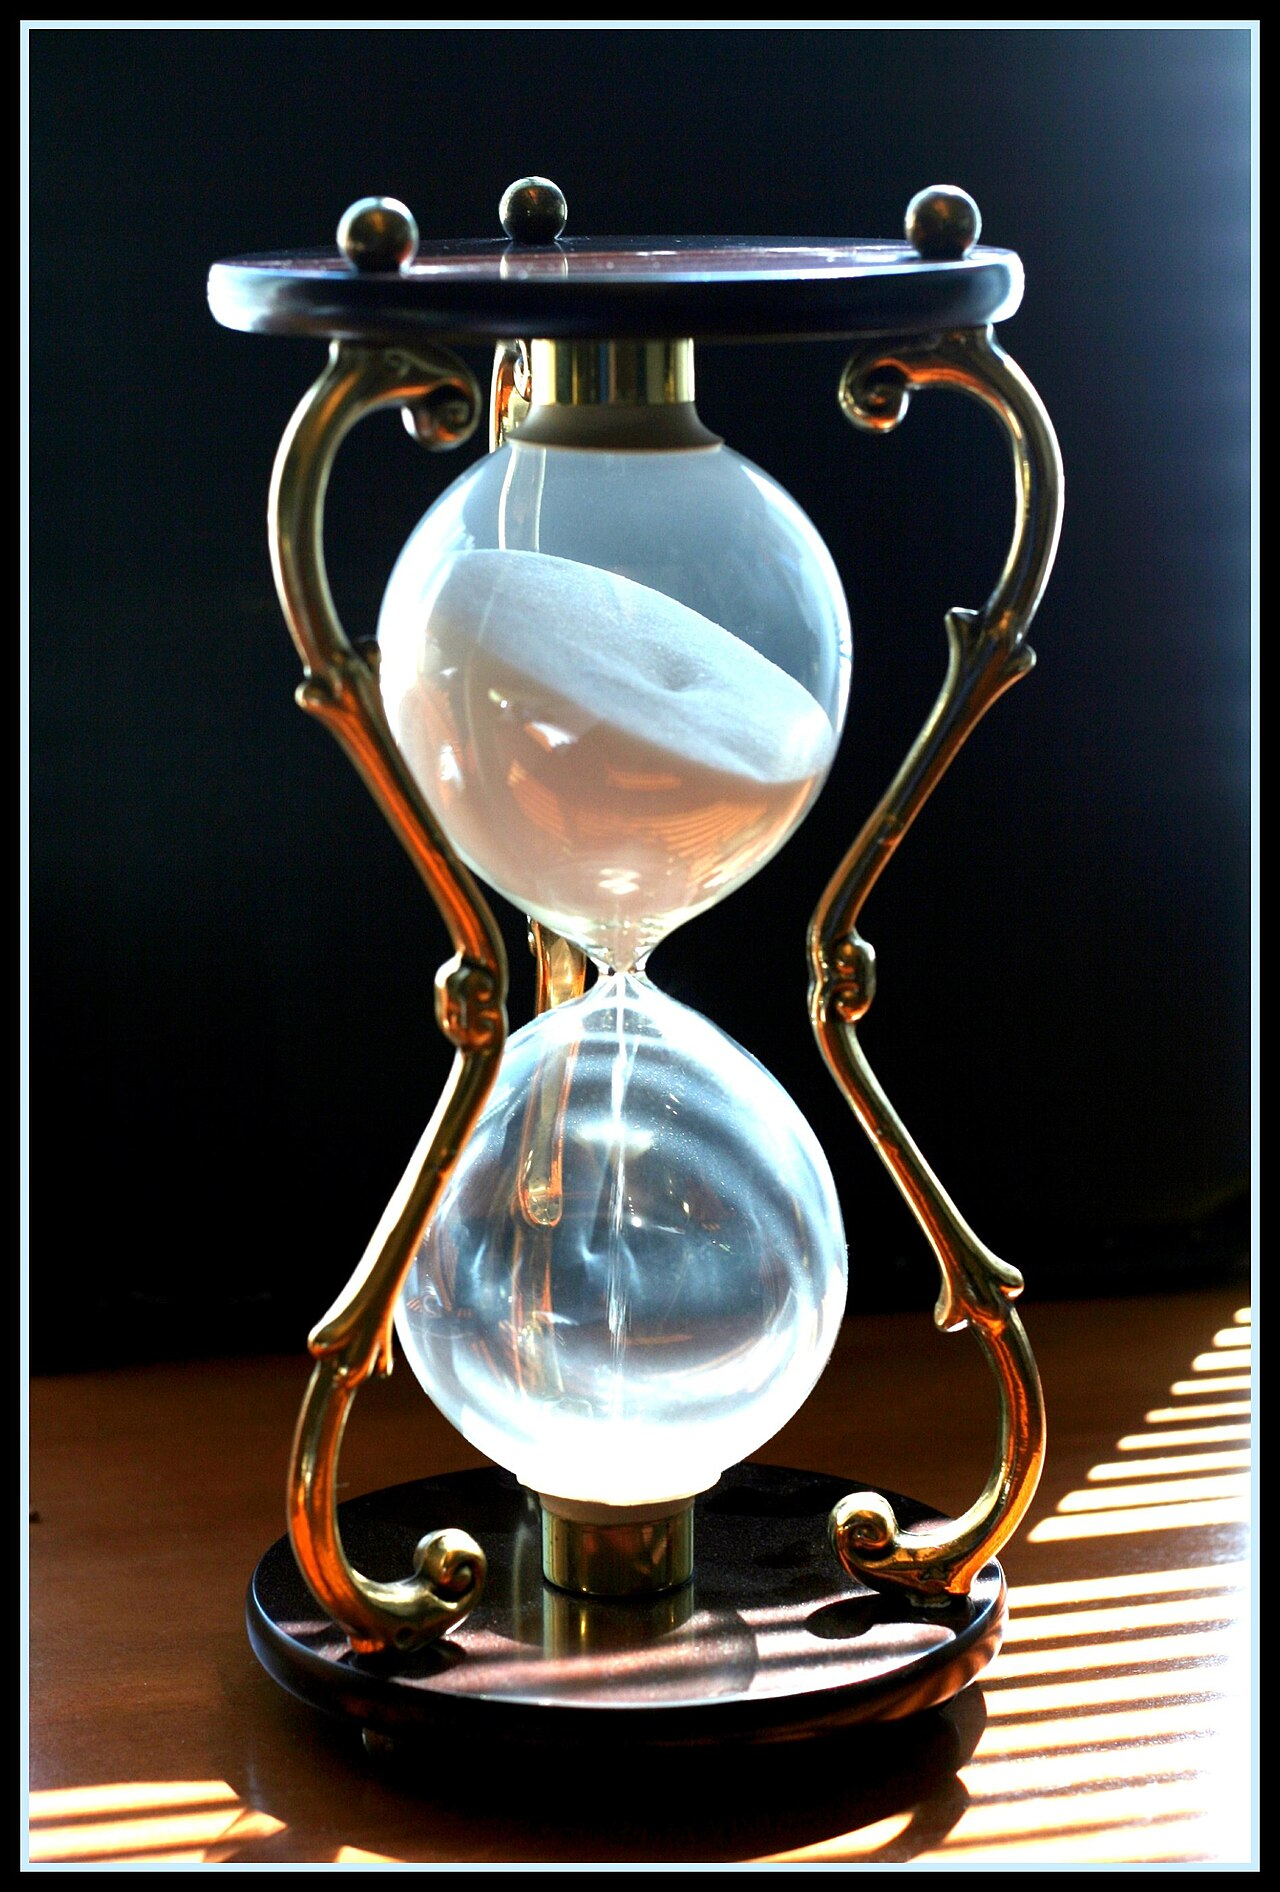
\includegraphics[width=0.34\linewidth]{images/book1/hourglass.jpg}

{\small ساعة رملية: \omterm{def:g2:measuring-time:duration}{مدة} تستطيع أن تمسكها بيدك. يحتاج الرمل إلى
الزمن نفسه دائمًا لينسلّ من الخصر الضيّق --- اقلبها فتحكم من
جديد. \emph{الصورة: جون مورغان،
CC BY 2.0.}}
\end{omfigure}

\begin{remark}[المشاعر ساعات رديئة]\label{rem:g2:measuring-time:feelings}
يطير بعد الظهر الممتع؛ ويزحف الطابور المملّ --- ومع ذلك قد تعدّ
الساعة لهما العدد نفسه. فإحساسنا بالزمن سهل الخداع، مثلما خُدع
اللمس في الساخن والبارد. ولهذا بالضبط تهمّ حكّام مثل الساعة
الرملية: فالرمل لا يملّ.
\end{remark}

\section{عدّ نبضات منتظمة}

\begin{definition}[الثانية]\label{def:g2:measuring-time:second}
\emph{الثانية}\index{ثانية} \omterm{def:g2:measuring-length:measure}{وحدة} الزمن المستعملة في العالم كله،
وتُكتب \unit{s}. والثانية الواحدة نحو نبضة قلب هادئة، أو دقّة
منتظمة من ساعة كبيرة. وقولك ``تمساح صغير واحد، تمساحان صغيران''
على مهل يعدّ ثانية واحدة تقريبًا لكل تمساح.
\end{definition}

\begin{example}[جرّب: كم ثانية؟]\label{ex:g2:measuring-time:count}
عُدّ الثواني بانتظام بينما: تحبس نفَسك حبسًا مريحًا؛ ويملأ
الصنبور كأسًا؛ ويجري صديق إلى السياج ويعود. قد يستغرق ملء الكأس
$6$ ثوانٍ، والجري $20$. والآن يمكن أن ينال تنظيف الأسنان والأغنية
\emph{أعدادًا} --- والأعداد، كما في الأطوال، تستطيع أن تسافر وأن
يُتحقّق منها.
\end{example}

\begin{example}[الساعات على الساعة]\label{ex:g2:measuring-time:clock}
الثواني للأشياء القصيرة. أما الامتدادات الطويلة فتُعدّ
\emph{بالساعات}\index{ساعة}: فصباحات المدرسة تدوم ساعات، وليلة
النوم كذلك. والعقرب القصير في الساعة يشير إلى الساعة: فإن كان على
العدد $3$ تمامًا فالوقت الثالثة؛ وإن كان بين $3$ و$4$ والعقرب الطويل
يشير إلى الأسفل تمامًا فالوقت الثالثة والنصف. واليوم بنهاره وليله
معًا يسع $24$ ساعة --- بينما تتمّ الأرض، كما تذكر، دورة كاملة.
\end{example}

\begin{omfigure}
\begin{tikzpicture}[scale=0.85]
  \draw[thick] (0,0) circle (1.5);
  \foreach \h in {1,...,12} {
    \node[font=\footnotesize] at ({90-\h*30}:1.22) {\h};
  }
  \draw[very thick, omDef] (0,0) -- ({90-3*30}:0.8);
  \draw[thick, omThm] (0,0) -- (90:1.05);
  \node[below, font=\small] at (0,-1.75) {الثالثة تمامًا};
  \begin{scope}[xshift=6cm]
    \draw[thick] (0,0) circle (1.5);
    \foreach \h in {1,...,12} {
      \node[font=\footnotesize] at ({90-\h*30}:1.22) {\h};
    }
    \draw[very thick, omDef] (0,0) -- ({90-3.5*30}:0.8);
    \draw[thick, omThm] (0,0) -- (270:1.05);
    \node[below, font=\small] at (0,-1.75) {الثالثة والنصف};
  \end{scope}
\end{tikzpicture}

{\small ساعتان: العقرب القصير يدلّ على الساعة. وعند الثالثة
والنصف يكون قد قطع نصف الطريق من $3$ نحو $4$.}
\end{omfigure}

\section{تمارين}

\begin{exercise}[$\star$]\label{exo:g2:measuring-time:1}
رتّب: العشاء؛ \ الاستيقاظ؛ \ لعب بعد الظهر؛ \ الفطور؛
\ النوم.
\end{exercise}

\begin{exercise}[$\star$]\label{exo:g2:measuring-time:2}
لحظة أم \omterm{def:g2:measuring-time:duration}{مدة}؟ ``يقرع الجرس عند الظهر''؛ \ ``تُخبز الكعكة نصف
ساعة''؛ \ ``رحلنا بعد الغداء''؛ \ ``بدت الرحلة بلا نهاية''.
\end{exercise}

\begin{exercise}[$\star$]\label{exo:g2:measuring-time:3}
أُشعلت شمعتان في اللحظة نفسها؛ فانطفأت الحمراء والزرقاء ما زالت
تشتعل. أيّ الشمعتين دامت أطول؟ وأيّ قاعدة من
\cref{met:g2:measuring-time:race} اتّبعتها الشمعتان؟
\end{exercise}

\begin{exercise}[$\star$]\label{exo:g2:measuring-time:4}
لماذا تكون الساعة الرملية حكمًا عادلًا للمُدد؟ وما الذي يبقى
فيها واحدًا في كل مرة تُقلب؟
\end{exercise}

\begin{exercise}[$\star$]\label{exo:g2:measuring-time:5}
يقول بن إن انتظاره المملّ عند طبيب الأسنان دام ``إلى الأبد''.
وتقول ساعته إنه دام أقلّ من فيلمه المتحرّك المفضّل. كيف يكون
هذا؟ (انظر \cref{rem:g2:measuring-time:feelings}.)
\end{exercise}

\begin{exercise}[$\star$]\label{exo:g2:measuring-time:6}
عُدّ الثواني بانتظام وقِس: كم ثانية تستغرق لتكتب اسمك كاملًا؟
ولتلبس حذاءك؟
\end{exercise}

\begin{exercise}[$\star$]\label{exo:g2:measuring-time:7}
أيّ \omterm{def:g2:measuring-length:measure}{وحدة} أنسب، الثواني أم الساعات: عطسة؛ \ ليلة نوم؛ \ ربط رباط
حذاء؛ \ صباح مدرسي؟
\end{exercise}

\begin{exercise}[$\star$]\label{exo:g2:measuring-time:8}
ارسم ساعة تشير إلى الخامسة تمامًا، وأخرى تشير إلى الخامسة
والنصف. إلى أين يشير العقرب القصير عند الخامسة والنصف؟
\end{exercise}

\begin{exercise}[$\star\star$]\label{exo:g2:measuring-time:9}
حمّام الأمس ودشّ اليوم لا يستطيعان أن يتسابقا. اشرح خطوة خطوة
كيف تعرف أيّهما أطول باستعمال ساعة رملية واحدة --- وماذا تكتب
حتى يتحقّق منه صديقك.
\end{exercise}

\begin{exercise}[$\star\star$]\label{exo:g2:measuring-time:10}
تعدّ ليلى ``واحد، اثنان، ثلاثة\dots'' بسرعة كبيرة فتقول إن الكأس
امتلأ في $12$ ثانية؛ ويعدّ توم على مهل فيجد $6$. وقد جرى الصنبور
جريانه نفسه في المرتين. مَن أقرب إلى الحقيقة، وما الذي يجعل عدّ
الثواني أمينًا؟
\end{exercise}
